\chapter{Revised Object-Oriented Structural Analysis Program}

\section{Introduction}
Assignment 4 extends the Assignment 3 object-oriented Direct Stiffness Method (DSM) solver to include two additional physical actions: thermal loading and support settlement. The extension is intentionally conservative in software architecture and mathematical formulation: thermal actions are modeled through equivalent nodal loads (fixed-end effects) and therefore do not modify the global stiffness matrix, while support settlements are modeled as prescribed displacements and solved through the partitioned DSM equations.

This separation is not only mathematically consistent but also critical for software continuity. Thermal effects are introduced as load-vector contributions generated at element level, whereas settlements alter boundary conditions and appear in the global system through restrained displacement terms. The same class backbone, assembly process, and solve-recover workflow from Assignment 3 are retained. Consequently, backward compatibility is preserved: when thermal loads are absent and prescribed settlements are zero, the solver behavior reduces to the original Assignment 3 implementation.

The objective of this chapter is to justify these design choices and document how the new capabilities were integrated without changing the core architecture.

\pagebreak
\section{Analysis and Design Decisions}

\subsection{Thermal vs Settlement Modeling}

Thermal actions and support settlements require different treatments because they enter the DSM equations in different ways. Thermal effects originate as strain-induced member actions, so they are transformed into element fixed-end forces and assembled into the global load vector. Settlements are imposed kinematic constraints at supports, so they are introduced as prescribed restrained displacements in the partitioned global equations.

This distinction ensures that:

\begin{itemize}
    \item Thermal effects are handled locally within element formulations
    \item Settlement effects are handled globally through system partitioning
\end{itemize}

A unified \texttt{TemperatureLoad} representation was adopted with fields $T_{\text{uniform}}$, $T_{\text{top}}$, and $T_{\text{bottom}}$ to avoid duplicating load definitions across element types and to keep the load abstraction consistent. Element-specific behavior is handled polymorphically (\texttt{FrameElement} vs. \texttt{TrussElement}), where frame elements generate both axial and bending effects while truss elements retain axial-only behavior. This design improves extensibility at the cost of requiring conditional handling within element implementations.

\subsection{Modification Strategy}

The solver was extended using the following approach:

\begin{itemize}
    \item The \texttt{Material} class was extended to include the coefficient of thermal expansion $\alpha$
    \item The \texttt{Section} class was extended to include section depth $d$ for thermal gradient calculations
    \item The \texttt{Node} class was extended to store prescribed displacements
    \item The \texttt{FrameElement} and \texttt{TrussElement} classes were extended to compute thermal fixed-end forces
    \item The \texttt{Structure} class was extended to solve the partitioned system for settlement
\end{itemize}

The placement of parameters follows physical ownership: $\alpha$ is a material property, depth $d$ is a section property, prescribed settlements are nodal boundary data, and the partitioned solution belongs to the global \texttt{Structure} solve stage. This preserves separation of concerns, minimizes disruption to the Assignment 3 codebase, and keeps the extension traceable.

When prescribed settlements are zero, the settlement formulation gives
\begin{equation}
K_{ff}u_f = F_f,
\end{equation}
which is exactly the Assignment 3 free-DOF system.

\pagebreak
\section{Module Change Table}

\begin{table}[H]
    \centering
    \caption{Module/Class changes introduced in Assignment 4}
    \label{tab:module_change_table}
    \renewcommand{\arraystretch}{1.25}
    \setlength{\tabcolsep}{4pt}
    \begin{tabular}{p{0.18\textwidth}p{0.31\textwidth}p{0.43\textwidth}}
        \toprule
        Module / Class & Modification & Rationale \\
        \midrule
        Material & Added thermal expansion coefficient $\alpha$ & Thermal strain is a material law parameter \\
        Section & Added depth $d$ & Thermal gradient curvature depends on section depth \\
        Node & Added prescribed displacement storage & Settlements are nodal boundary conditions \\
        FrameElement & Added thermal fixed-end force evaluation (axial + bending) & Frame members carry axial and flexural thermal effects \\
        TrussElement & Added thermal fixed-end force evaluation (axial only) & Truss members carry axial force only \\
        Structure & Added partitioned solve terms with restrained displacements & Settlements modify global RHS through $-K_{fr}u_r$ \\
        \bottomrule
    \end{tabular}
    \renewcommand{\arraystretch}{1.0}
    \setlength{\tabcolsep}{6pt}
\end{table}

\pagebreak
\section{Revised UML and Class Modifications}

\subsection{Updated Class Responsibilities}

Class responsibilities were refined but not restructured. \texttt{Material} owns $\alpha$, \texttt{Section} owns $d$, \texttt{Node} owns prescribed displacements, element classes compute local thermal fixed-end contributions, and \texttt{Structure} owns global partitioning and solution. This allocation keeps each class responsible for data and operations at its natural abstraction level.

\subsection{UML/Class Diagram}

The UML reflects targeted extensions rather than architectural replacement. The inheritance backbone is preserved exactly as in Assignment 3, with \texttt{Element} as base class and \texttt{FrameElement}/\texttt{TrussElement} as specialized subclasses. No new parallel hierarchy was introduced; only relevant attributes/methods were added to existing classes.

\begin{figure}[H]
    \centering
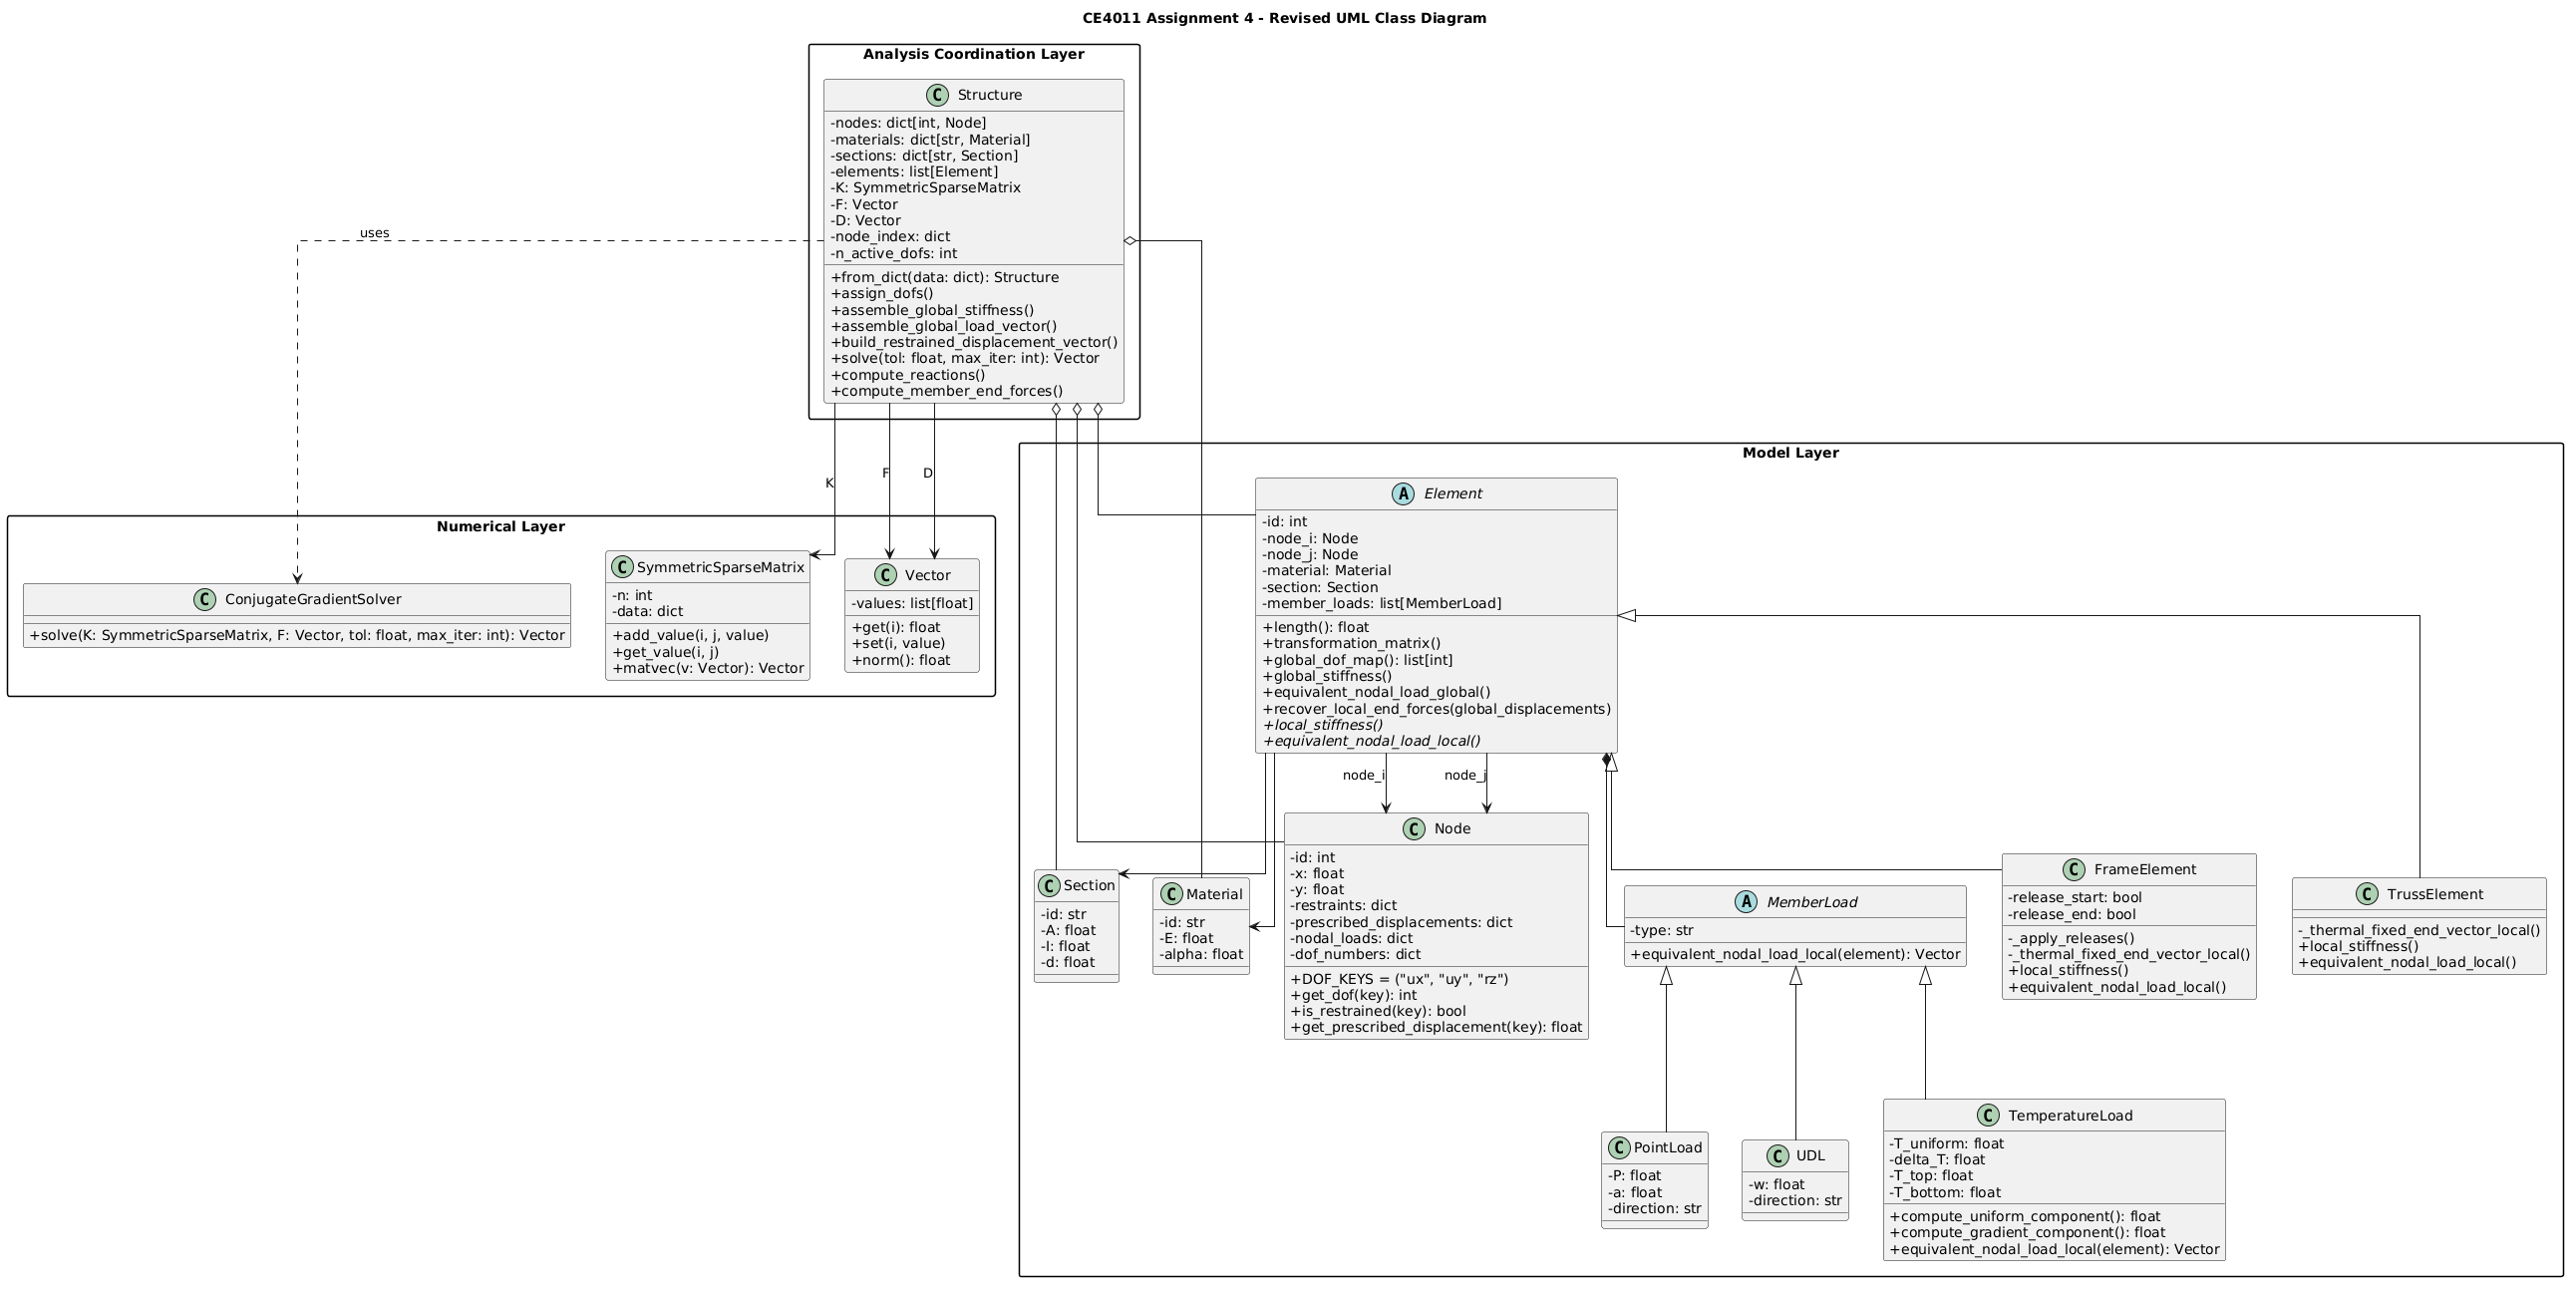
\includegraphics[width=0.95\textwidth,height=0.58\textheight]{UML_4.png}
    \caption{Revised UML/Class Diagram showing thermal and settlement extensions}
    \label{fig:uml_assignment4}
\end{figure}

\subsection{Updated Relationships for Thermal and Settlement Effects}

Assignment 4 adds thermal loading and settlement handling without changing the core
object model. The main relationship updates affect \texttt{Element},
\texttt{FrameElement}, and \texttt{Structure}.

\subsubsection{Element--Thermal Load Relationship}

Each \texttt{Element} composes thermal load data and normalizes it into:
\begin{itemize}
    \item Uniform temperature change ($T_{\text{uniform}}$)
    \item Temperature gradient ($\Delta T$)
\end{itemize}

These parameters are converted to equivalent fixed-end forces in local coordinates
before global assembly, consistent with DSM load treatment.

\subsubsection{FrameElement Specialisation}

\texttt{FrameElement} supports axial and flexural thermal effects:
\begin{itemize}
    \item Uniform temperature change produces axial forces:
    \[
    N_t = EA \alpha T_{\text{uniform}}
    \]
    \item Temperature gradients produce bending moments:
    \[
    M_t = \frac{EI \alpha \Delta T}{d}
    \]
\end{itemize}

These contributions are added to the local fixed-end vector and transformed during
assembly. By contrast, \texttt{TrussElement} remains axial-only, so thermal-gradient
bending is ignored.

\subsubsection{Structure--Prescribed Displacement Relationship}

Support settlements are modeled as non-zero prescribed displacements at constrained
DOFs. The partitioned system is:

\[
\begin{bmatrix}
K_{ff} & K_{fc} \\
K_{cf} & K_{cc}
\end{bmatrix}
\begin{bmatrix}
d_f \\
d_c
\end{bmatrix}
=
\begin{bmatrix}
F_f \\
F_c
\end{bmatrix}
\]

with $d_f$ as unknown free DOFs and $d_c$ as prescribed displacements. The reduced
equation is:

\[
K_{ff} d_f = F_f - K_{fc} d_c
\]

so settlement effects enter the RHS while preserving the global stiffness formulation.

\subsubsection{Updated Relationship Summary}

The extension preserves Assignment 3 architecture while adding:

\begin{itemize}
    \item Element now composes thermal load definitions
    \item FrameElement includes thermal force and moment generation
    \item Structure handles prescribed displacements through system partitioning
\end{itemize}

\begin{table}[H]
\centering
\caption{Updated class relationships in Assignment 4}
\begin{tabular}{llll}
\toprule
From & To & Type & Description \\
\midrule
Element & Thermal Load & Composition & Element owns thermal load data \\
FrameElement & Thermal Effects & Specialisation & Generates axial and bending thermal effects \\
Structure & Prescribed DOF & Association & Handles non-zero displacement constraints \\
\bottomrule
\end{tabular}
\end{table}

\pagebreak
\section{Thermal Loading Extension}

\subsection{Modeling Approach}

Thermal effects are incorporated using fixed-end force equivalence. The element-level thermal strain field is converted into equivalent nodal actions and assembled into the global load vector. Therefore, thermal loading changes the right-hand side but not the global stiffness matrix.

\subsection{Uniform Temperature Change}

A uniform temperature change produces an axial strain:

\begin{equation}
\epsilon_{th} = \alpha \Delta T
\end{equation}

For a fully restrained member, this results in an axial force:

\begin{equation}
N_t = E A \alpha \Delta T
\end{equation}

This is the mean-temperature contribution and corresponds to an axial effect.

\subsection{Thermal Gradient Effects}

A temperature gradient across the section depth induces curvature:

\begin{equation}
\kappa = \alpha \frac{\Delta T}{d}
\end{equation}

The resulting bending moment is:

\begin{equation}
M_t = E I \alpha \frac{\Delta T}{d}
\end{equation}

This is the gradient-temperature contribution and corresponds to a bending effect.

\subsection{Implementation in Elements}

Thermal decomposition is implemented at element level:

\begin{itemize}
    \item Mean temperature component $\rightarrow$ axial thermal force
    \item Gradient component $\rightarrow$ bending thermal moment
\end{itemize}

Frame elements can carry both thermal axial force and thermal bending moment. Truss elements carry only thermal axial force, with no thermal bending terms.

\pagebreak
\section{Support Settlement Extension}

\subsection{Settlement Modeling Approach}

Support settlements are modeled as prescribed displacements at restrained degrees of freedom. Unlike thermal effects, settlement is not an element load; it modifies boundary kinematics and enters the partitioned global equations.

\subsection{Partitioned System Formulation}

The global stiffness equation is partitioned as:

\begin{equation}
\begin{bmatrix}
K_{ff} & K_{fr} \\
K_{rf} & K_{rr}
\end{bmatrix}
\begin{Bmatrix}
u_f \\
u_r
\end{Bmatrix}
=
\begin{Bmatrix}
F_f \\
F_r
\end{Bmatrix}
\end{equation}

For non-zero prescribed displacements, the system is solved as:

\begin{equation}
K_{ff} u_f = F_f - K_{fr} u_r
\end{equation}

Support reactions are obtained from:

\begin{equation}
F_r = K_{rf} u_f + K_{rr} u_r
\end{equation}

In implementation, \texttt{Structure} constructs $u_r$ from nodal prescribed displacement data and applies settlement by modifying the right-hand side with the $-K_{fr}u_r$ term before solving for $u_f$.

\pagebreak
\section{Updated Relationships and Workflow}

\begin{figure}[H]
    \centering
    
\includegraphics[width=0.85\textwidth]{ActivityDiagram.png}
    \caption{Updated analysis workflow incorporating thermal and settlement effects}
    \label{fig:workflow_assignment4}
\end{figure}

\pagebreak
\section{Input Format}

\subsection{Data Schema Overview}

The solver supports both JSON and XML inputs. In both formats, thermal actions are defined at element/member-load level, while settlements are defined as prescribed displacements at restrained nodal DOFs.

\subsection{Example Input Snippet}

\begin{lstlisting}[language=XML,caption={Example XML snippet from ModelB thermal case},label={lst:input_snippet}]
<structure>
    <nodes>
        <node id="2" x="7.0" y="8.0">
            <restraints ux="false" uy="false" rz="false" />
        </node>
    </nodes>

    <elements>
        <element id="1" type="frame" node_i="1" node_j="2" material="concrete" section="beam">
            <member_loads>
                <thermal T_top="0.0" T_bottom="50.0" />
            </member_loads>
        </element>
        <element id="3" type="truss" node_i="4" node_j="2" material="steel" section="pipe">
            <member_loads>
                <thermal T_uniform="50.0" />
            </member_loads>
        </element>
    </elements>
</structure>
\end{lstlisting}

\pagebreak
\section{Output Format}

\subsection{Reported Quantities}

The solver produces the following outputs:

\begin{itemize}
    \item Nodal displacements
    \item Support reactions
    \item Member-end forces in local coordinates
\end{itemize}

\subsection{Output Table Structure}

\begin{table}[H]
    \centering
    \caption{Output quantities}
    \label{tab:output_quantities}
    \begin{tabular}{lll}
        \toprule
        Quantity & Unit & Description \\
        \midrule
        Displacement & m, rad & Nodal DOFs \\
        Reaction & N, Nm & Support forces and moments \\
        Member-end forces & N, Nm & Local element forces \\
        \bottomrule
    \end{tabular}
\end{table}

\pagebreak
\section{File Structure}

The Assignment 4 project is organized into a modular directory structure to
separate source code, input data, testing, results, and documentation. This
organization improves maintainability, readability, and reproducibility of the
analysis workflow.

GitHub repository: \url{https://github.com/ImranMETU/CE4011_Assignment4}

\subsection{Top-Level Directory Structure}

\begin{verbatim}
Assignment4/
|
|-- benchmark/          # Benchmark models and exports (FTOOL/SAP2000)
|-- docs/               # Supporting documentation and notes
|-- inputs/             # Input files for analysis (XML/JSON)
|-- report/             # LaTeX report files (main.tex, chapters, figures)
|-- results/            # Solver outputs and comparison results
|-- scripts/            # Execution scripts (run_thermal, run_model_b, etc.)
|-- settlement/         # Settlement-specific cases and utilities
|-- thermal/            # Thermal load utilities and related modules
|-- src/                # Core solver implementation
|-- tests/              # Unit, interface, and regression tests
|
|-- .gitignore          # Git ignore rules
`-- README.md           # Project overview and usage instructions
\end{verbatim}

\subsection{Directory Description}

\begin{itemize}
    \item \textbf{src/}: Contains the core object-oriented implementation of the
    structural analysis solver, including element definitions, material models,
    and global assembly routines.

    \item \textbf{thermal/}: Implements thermal load functionality, including
    temperature normalization, fixed-end force calculations, and equivalent
    nodal load generation.

    \item \textbf{settlement/}: Contains logic and utilities for handling
    prescribed displacements and support settlement effects.

    \item \textbf{scripts/}: Includes executable Python scripts used to run
    analysis cases, such as thermal simulations, regression tests, and
    assignment-specific models.

    \item \textbf{inputs/}: Stores structured input files defining geometry,
    materials, boundary conditions, and loads for different analysis cases.

    \item \textbf{tests/}: Provides unit, interface, and regression tests used
    to verify solver correctness and validate new features introduced in
    Assignment 4.

    \item \textbf{results/}: Contains solver outputs, processed results, and
    comparison data used for validation against benchmark software.

    \item \textbf{benchmark/}: Includes verification models and exported results
    for benchmark comparison (with subfolders such as \texttt{ftool/} and
    \texttt{sap2000/}).

    \item \textbf{report/}: Contains all LaTeX source files, figures, and tables
    required to generate the final report.

    \item \textbf{docs/}: Stores supplementary documentation, notes, or design
    references used during development.

    \item \textbf{README.md}: Provides instructions for running the solver,
    executing tests, and reproducing results.
\end{itemize}
